\documentclass{sig-alternate}

\usepackage{subfigure}

 


\begin{document}

\newcommand{\Cc}{\mathcal{C}}
\newcommand{\Vc}{\mathcal{V}}
\newcommand{\Ec}{\mathcal{V}}


%\conferenceinfo{The 4th SNA-KDD Workshop}{'10 ( SNA-KDD'10),July 25, 2010 , Washington D.C. USA}
\title{Studying  community growth in LiveJournal}
\numberofauthors{3} 
\author{
\alignauthor
Simla Ceyhan\\
       \affaddr{Management Science and Engineering}\\
       \affaddr{Stanford University}\\
       \email{simlac@stanford.edu}
\alignauthor
Shirin Jalali\\
       \affaddr{Center for Mathematics of Information}\\
       \affaddr{California Institute of Technology}\\
       \email{shirin@caltech.edu}}

\maketitle
\begin{abstract}
This paper studies growth of communities in LiveJournal which is  an online social network that has 
user-defined communities. The primary goal of this work is to find features of communities that affect their growth in the future.  We studied about $2000$ communities  inside LiveJournal, and collected data from them in 7 snapshots spanned in a period of five months.  That is for each community at each snapshot, we recorded its members and their friends lists inside LiveJournal.

For each member of a community, we define the notion of  \emph{attractiveness}, which reflects how successful she has been in attracting her friends to join the community. We find that the percentage of attractive members of a community in a short time interval, has a strong correlation with its growth rate in the future. We also tried to measure the correlation between the growth and some structural properties of the communities such as  clustering coefficient and average degree. None of them showed a similar evidence of strong correlation.

\end{abstract}

\category{H2.8}{Database Applications}{Data Mining}
\category{J.4}{Social and Behavioral Sciences}{Sociology}

\terms{Human Factors, Measurement}
\keywords{Social Networks, Community Growth}


\section{Introduction}

The process by which people get together and form communities has been an active area of research, at the intersection of psychology, sociology, and computer science \cite{social_ref}. The recent emergence of online social networks facilitates a data-driven approach to the study of this topic and can lead to exciting new insights about the behavior of individuals. 

Understanding the dynamics of communities is crucial as they give hints about the larger 
social network that they form. However, one challenge comes form the fact that it is difficult to
identify the underlying communities of a network \cite{newman, danon, www10}.  To overcome this challenge, 
we used an online social networking and blogging site, LiveJournal, as our primary source of data.
LiveJournal is not only a large social network but also it has a significant collection of explicitly
identified communities. By analyzing data that we have collected over a span of 5 months, we aim to answer mainly the following question:

\begin{itemize}
\item Can we predict whether a community will grow over time?
\end{itemize}

For studying the growth of communities we investigate several features such as clustering coefficient, and average degree. From our analysis, among the features we considered, the parameter that turns out to have the most significant effect is related to what we call $\emph{attractiveness}$. We define the notion of being attractive for members of a community. It reflects how successful each person has been in attracting his/her friends to join the community.

Using regression analysis, we show that there is a strong positive correlation between the percentage of attractive members of a community and its growth. We also tried to measure the correlation between the growth and some structural properties of the communities such as clustering coefficient and average degree. None of them showed evidence of strong correlation as \emph{percentage of attractive members} did. 

Later, in order to understand the notion of being attractive more, we looked at how it changes with over time or in different communities. Our data shows that among the newly joined members, the percentage of attractive members is much higher. People that are members of multiple communities tend to be attractive in most of them at the same time. Our last observation is that people are attractive for a short span of time.



\subsection{Related Literature}
Many studies on online social networks and biological
networks focused on properties of network evolution such as shrinking 
diameters and edge creation \cite{kumar_tomkins, LKF, micro_evol}.
These studies focus on understanding the change in the overall
network over time. On the other hand, the evolution of the 
underlying communities in a network has not been studied as much. 

There is also a large body of work on identifying the communities in 
networks \cite{newman, danon, www10}.
A community of a network or tightly connected clusters is typically thought of
as a group of nodes with more and/or better interactions amongst
its members than between its members and the remainder of the
network \cite{define_comm}. However, in our study, the communities are 
already explicitly identified. As mentioned before, our focus is understanding 
the mechanisms by which the communities grow.

A previous study that inspired this work is  Backstrom
et al. \cite{group_formation} paper, where the authors focus on the role of common
friends on a community's formation and growth. They use decision-tree techniques
to identify the properties of the social network that affect its evolution.

%COMPARE WITH OUR RESULTS?????????????????

\section{Network data}

As mentioned before, in this paper we focus on LiveJournal which is an  online social network with more than 19 million members.  It is an active social network with an average of 300,000 updates a day. 
Members maintain a blog, declare friends, and join communities. Thus there is a notion of a friendship graph, whose nodes correspond to users and edges correspond to friendship relationship. Let the undirected graph $\mathcal{G}=(\mathcal{V},\mathcal{E})$ represent the friendship structure among the members of LiveJournal. Each node $v\in\mathcal{V}$ represents one of the members, and each each edge $e=[v_1,v_2]\in\mathcal{E}$ shows that $v_1$ and $v_2$ are friends. 

There are different communities in LiveJournal. Each member can join as many communities as he/she desires. Each community $\mathcal{C}$ corresponds to a subgroup of the members of the LJ, and induces a subgraph $\mathcal{G}_{\mathcal{C}}=[\mathcal{C},\mathcal{E}_{\mathcal{C}}]$ of the main graph $\mathcal{G}$ such that  each edge $e=[v_1,v_2]\in\mathcal{E}$ with $v_1\in\mathcal{C}$ and  $v_2\in\mathcal{C}$ belongs to $\mathcal{G}_{\mathcal{C}}$ as well.

For this study, we followed the members of more than $2000$ communities, and  collected data over seven snapshots during a period of five months.  The time intervals between the snapshots is shown in Table \ref{tb:data}. At each snapshot, we recorded the  members of each of the 2000 communities. Moreover, for each  member, we registered his/her friends, both inside and outside the community. 

\begin{table}[htdp]
\begin{center}
\begin{tabular}{|c|c|}
\hline
Snapshot  & Time between the snapshot  \\
  & and its previous one \\ \hline
0 & -  \\ \hline
1 & 1 week \\ \hline
2 & 1 week \\ \hline
3 & 1 week \\ \hline
4 & 2 weeks \\ \hline
5 & 8 weeks \\ \hline
6 & 6 weeks \\ \hline
\end{tabular}
\end{center}\caption{Brief description of the data}
\label{tb:data}
\end{table}%



%\section{Some definitions}
 


\section{Analysis}

\subsection{Definitions} \label{sec: definitions}
For a community $\mathcal{C}$, the people who are not currently one of its members, but have at least one friend inside it are called its \emph{fringe}  \cite{group_formation} (refer to Fig. \ref{fig: fringe}).  
\begin{figure}
\begin{center}
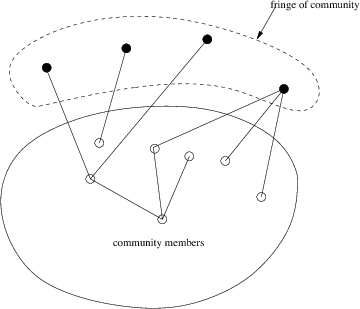
\includegraphics[width=50mm]{../figures/fringe.pdf}\caption{Fringe of a community}\label{fig: fringe}
\end{center}
\end{figure}
The reason for defining such group for each community  $\Cc$ is that those in the fringe of $\mathcal{C}$ are more probable to join it in the future compared to those who are not acquainted with anyone inside $\Cc$ \cite{group_formation}. Clearly the fringe of a community can change during time; Some people from the fringe join the community, and hence are removed from the fringe, some other people might become friends with some members of $\Cc$, and hence join its fringe.   Let $\mathcal{F}(t)$ denote the fringe of $\mathcal{C}$ at snapshot $t$.
Let $\mathcal{C}_{\mathcal{F}}(t)  \subset \mathcal{F}(t)$ denote people who 
were in the fringe of the community at snapshot $t-1$, but have joined it at snapshot  $t$ (refer to Fig. \ref{fig: evolution} where blue circles denote some members of $\mathcal{C}_{\mathcal{F}}(t)$).
\begin{figure}
\begin{center}
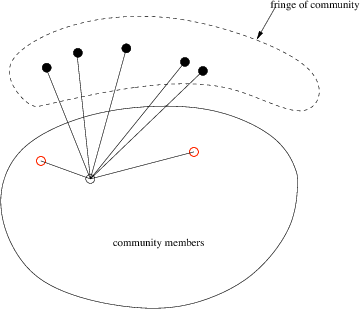
\includegraphics[width=50mm]{../figures/att_snapshot1.pdf}
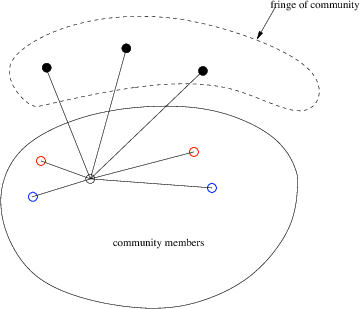
\includegraphics[width=50mm]{../figures/att_snapshot2.pdf}\caption{Community evolution between snapshots $t-1$ and $t$}\label{fig: evolution}
\end{center}
\end{figure}


For the members of each community $\Cc$ we define a notion of being attractive which reflects how successful each person has been in attracting his/her friends from the fringe to joining the community. More specifically, a user inside the community is called \emph{attractive} at snapshot $t$, if the  percentage of his/her friends who have joined the community in the time interval between  snapshot $t-1$ till snapshot $t$  is larger than the average, i.e., the fraction of the total number of people in the fringe who have joined the community during the same period (refer to Fig. \ref{fig: evolution}).  Therefore, for a user $v\in\mathcal{C}$, 
\begin{align}
a_v\triangleq
\left\{\begin{array}{cc}      
                   1 & \textmd{ if }  \frac{|\partial v 
                   \cap \mathcal{C}_{\mathcal{F}}(t)|}
                   { |\partial v \cap  \mathcal{F}(t)|}> 
                   \frac{|\mathcal{C}_{\mathcal{F}}(t)|}{|\mathcal{F}(t)|}\\  
                   0 & \textmd{ otherwise },
                   \end{array}
\right.
\end{align}
where $\partial v$ denotes the set of friends of $v$, i.e., $\partial v=\{v'\in\mathcal{V}: \;\; [v,v']\in\Ec\}$, and for two arbitrary sets $A$  and $B$, $A \cap B$ denotes their intersection. 
Note that this definition is both group and time dependent. It means that a user might be considered attractive in some community and unattractive in some other community. Also, it might be labeled as attractive during some time interval, and unattractive during some other time interval.

In this paper, we also define  a notion of sociability.  A user $v$ is called \emph{social} if  her degree is larger than the average degree of the graph, i.e.,
\begin{align*}
                   s_v=\left\{\begin{array}{cc}
                   1 & \textmd{ if } |\partial v|>d_{\rm av}\\
                   0 & \textmd{ o.w. },
                   \end{array}
                   \right.
\end{align*}
where for a set $A$, $|A|$ denotes its size. Note that each user is either social or asocial and this does not depend on the groups she belongs too.







\subsection{Observation} \label{sec: initial}
%\subsubsection{Is community growth affected by the number of attractive members?}
Our main goal in this paper is to study evolution of communities residing inside a social network. In particular, we are interested in understanding what parameters affect the growth of a community. In Section \ref{sec: definitions}, 
for the members of a community $\Cc$, we defined the notion of being attractive. In this section, we provide some initial observations connecting the percentage of attractive members of a community to its growth. In Section \ref{sec: regression},  these elementary observations are supported by  regression analysis. 


The growth rate of a community $\Cc$ at snapshot $t$ is defined as
\begin{align}
r_g(t,\Cc) = \frac{|\mathcal{C}_{\mathcal{F}}(t)|}{|\mathcal{C}(t)|},
\end{align}
Let $\bar{r}_g(t)$ denote the average growth rate of the communities under study at snapshot $t$. At each snapshot, we divide the communities into two categories: \emph{growing} and \emph{non-growing}, based on their growth rate at that snapshot.  A community is called growing at snapshot $t$, if its growth rate in that snapshot is larger than the average, i.e., $r_g(t,\Cc) \geq \bar{r}_g(t)$. Otherwise, it is called non-growing.  

For each community $\Cc$, let $p_a(t,\Cc)$ denote the fraction of attractive members of the community at snapshot $t$, i.e.,
\begin{align}
p_a(t,\Cc) = \frac{\sum\limits_{v\in\Cc} a_v}{|\Cc|}.
\end{align}

Fig. \ref{fig: perc_att} shows the fraction of attractive members of growing and non-growing communities for 5 snapshots. 
\begin{figure}
\begin{center}
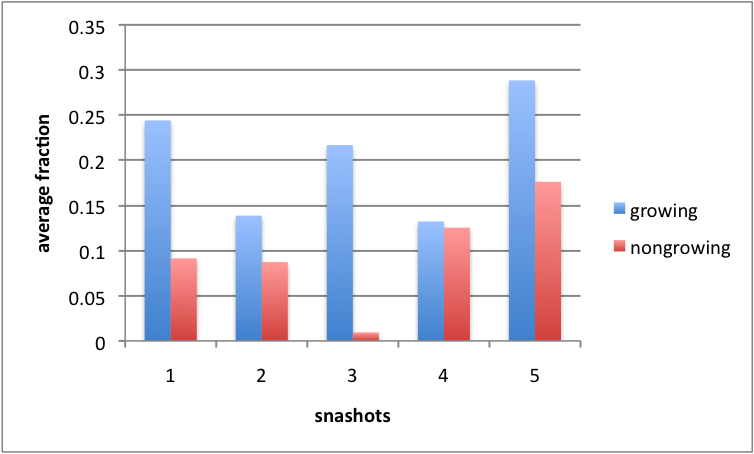
\includegraphics[width=80mm]{../figures/att_growth.png}\caption{Average percentage of attractive members for  growing and non-growing communities in 5 snapshots.}\label{fig: perc_att}
\end{center}
\end{figure}
It can be observed that in all cases the growing communities have on average higher percentage of attractive members. In the next section, we further investigate this observation which demonstrates  some positive correlation between the percentage of  attractive members of a community and its growth.
 



%\begin{figure}
%\begin{center}
%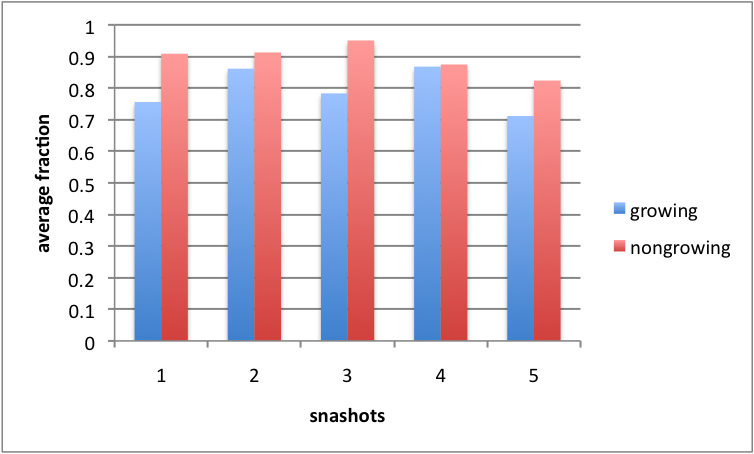
\includegraphics[width=80mm]{../figures/nonatt_growth.png}\caption{Percentage of unattractive members of growing and non-growing communities.}\label{fig: perc_unatt}
%\end{center}
%\end{figure}



\subsection{Regression analysis}\label{sec: regression}
In this section we present some regression analysis results for studying the dependence of a community's growth rate, $r_g(\Cc)$, on its percentage of attractive members. As mentioned before, our primary  goal is to determine  factors that affect the growth of a community in the future.  As we will show in this section through our regression analysis, there is a strong  positive correlation between the two.

Remember that the time span between the snapshots is shown in Table \ref{tb:data}. For each snapshot $t\in\{1,\ldots,6\}$ and for each community $\Cc$, we compute the following parameters: the fraction of attractive members of community $\Cc$ at snapshot $t$, i.e., $p_a(t,\Cc)$,  and its growth rate $r_g(t,\Cc)$, In addition to these time variant parameters, for each community we compute its average clustering coefficient $c_i$ \cite{clustering}, average degree $d_i$, and the percentage of \emph{social} people $p_s(\Cc)$ defined as
\begin{align}
p_s(\Cc) = \frac{\sum\limits_{v\in\Cc}s_v}{|\Cc|}.
\end{align}

As the first example, let us consider the following hypothesis,
\begin{align}
r_g(3,\Cc) = \alpha_{1,3}  p_a(1,\Cc) + n_{\Cc},\label{eq:reg1}
\end{align}
which predicts a linear dependence of $r_g(3,\Cc)$ on $p_a(1,\Cc)$.  In \eqref{eq:reg1} , $n_{\Cc}$ represents an independent Gaussian noise distributed as  $n_{\Cc} \sim N(0,\sigma^2)$. The analysis of variance (anova) analysis table generated by R is shown in Table \ref{tb:anova_g3_vs_a1}. The fitted coefficient is $\hat{\alpha}_{1,3}=0.2903$, and the last column of the table shows how significant this coefficient is. In order to give a picture of this linear correlation, Fig.4 shows  growth rates $r_g(3,\Cc)$  versus percentages of attractive members $p_a(1,\Cc)$ in a log scale for the communities which have a positive growth rate.
\begin{figure}
\begin{center}
\includegraphics[width=9cm]{../figures/gr3_vs_att1.pdf}
\caption{$r_g(3,\Cc)$ versus $p_a(1,\Cc)$ for communities with positive growth rate in a log basis}
\end{center}
\label{fig:g5_vs_a1}
\end{figure}

\begin{table}
\caption{Anova table: \texttt{lm($r_g(3,\Cc) \sim p_a(1,\Cc)$)}, fitted coefficient = $0.2903$}
\begin{center}
\begin{tabular}{c|c|c|c|c|c}
    &  Df  & Sum Sq & Mean Sq & F value &   Pr($>$F) \\ \hline
att1     &{\small  1 }& {\small 0.050669} & {\small 0.050669}  & {\small 286.16} &  $<$ {\small 2.2e-16 ***}\\ \hline
Res. & {\small 511} & {\small 0.090479} & {\small 0.000177}  & &
\end{tabular}
\end{center}
\label{tb:anova_g3_vs_a1}
\end{table}





\begin{table}
\caption{Anova table: \texttt{lm($r_g(5,\Cc) \sim p_a(2,\Cc)$)}, fitted coefficient = $0.3130$}
\begin{center}
\begin{tabular}{c|c|c|c|c|c}
         &  Df  & Sum Sq & Mean Sq & F value &   Pr($>$F)    \\ \hline
att2 &    1 & 0.03347 & 0.03347 & 19.058 & 1.574e-05 ***\\ \hline
Res. & 451 & 0.79199 & 0.00176 & \\
\end{tabular}
\end{center}
\label{tb:anova_g5_vs_a2}
\end{table}






Tables \ref{tb:anova_g5_vs_a2} to \ref{tb:anova_g6_vs_a5} show anova tables derived by performing similar analyses for some other snapshots.   In each case the growth rate in one snapshot is regressed against the percentage of attractive members in one of its previous snapshots. More specifically Table \ref{tb:anova_g5_vs_a2} contains anova analysis for testing $r_g(5,\Cc) = \alpha_{2,5} p_a(2,\Cc) + n_{\Cc}$, Table \ref{tb:anova_g5_vs_a3} reflects test results for $r_g(5,\Cc) = \alpha_{3,5} p_a(3,\Cc) + n_{\Cc}$, and Table \ref{tb:anova_g6_vs_a5} shows anova analysis for testing $r_g(6,\Cc) = \alpha_{5,6} p_a(5,\Cc) + n_{\Cc}$. The corresponding fitted coefficients are $\hat{\alpha}_{2,5}=0.3130$, $\hat{\alpha}_{3,5}=0.2624$, and $\hat{\alpha}_{5,6}=0.1651$. It can be observed that the fitted coefficients are in the range of $[1.5,3.5]$, and are  consistent. Moreover, the anova tables in all four cases state the significance of the fitted coefficients. 

One other parameter that can be considered as a potential candidate for predicting the growth of a community $\Cc$ is the clustering coefficient of its  induced graph $\mathcal{G}_{\Cc}$. To check this we test the following hypothesis: $r_g(3,t) = \beta_3  c_{\Cc} + n_{\Cc}$, where again $n_{\Cc}$ represents independent additive white Gaussian noise. The fitted coefficient and the anova analysis results are shown in Table \ref{tb:anova_g3_vs_cc}.   The fitted coefficient is $\hat{\beta}= 0.0130 $, but, according to the table, does not seem to of significance.


One other parameter of potential relevance is the average degree among the members of the community. Remember that we defined a person's sociability in terms of its degree. Therefore, the average degree of a community reflect on average how social its members are. To perform a test to check this dependence, we try $r_g(3,\Cc) = \gamma_3  \bar{d_{\Cc}} + n_i$ where $\bar{d}_{\Cc}$ denotes the average degree in community $\Cc$. The anova analysis is shown in Table \ref{tb:g3_vs_d}. The fitted coefficient is $\hat{\beta}=0.00086$ which again does not have any significance.


Finally as a sanity check we consider predicting the growth rate of a community based on its growth rate in one of the previous snapshots.  As an example of such analysis, Table \ref{tb:anova_g6_vs_g1} shows the anova table generated by R for checking $r_g(3,\Cc) = \eta_{1,3}  r_g(1,\Cc) + n_{\Cc}$ where $n_i\sim N(0,\sigma^2)$. Here the fitted coefficient turns out to be $\hat{\eta}_{1,3}=-0.1408$ which is negative. This shows the difference between the growth rate and percentage of attractive members. While the growth rate at some snapshot fails to predict the growth rate at future snapshots, the percentage of attractive members seems to be a reasonable factor to consider. To demonstrate pictorially how $r_g(1,\Cc)$ fails to predict $r_g(3,\Cc),$ Fig.~\ref{fig:g3_vs_g1} shows $r_g(3,\Cc)$ versus $r_g(1,\Cc)$ for 1111 communities that have $|r_g(1,\Cc)|<0.1$ and $|r_g(3,\Cc)|<0.1$.
\begin{figure}
\begin{center}
\includegraphics[width=90mm]{../figures/gr3_vs_gr1.pdf}\caption{$r_g(3,\Cc)$ versus $r_g(1,\Cc)$}\label{fig:g3_vs_g1}
\end{center}
\end{figure}
 It can be observed that the points are almost uniformly distributed around zero.




\begin{table}
\caption{Anova table: \texttt{lm($r_g(5,\Cc) \sim p_a(3,\Cc)$)}, fitted coefficient = $0.2624$}
\begin{center}
\begin{tabular}{c|c|c|c|c|c}
         &   {\small Df}  &  {\small Sum Sq} &  {\small Mean Sq }&  {\small F value} &   {\small  Pr($>$F)}    \\ \hline
 {\small att3}  &     {\small 1} &  {\small 0.02995} &  {\small 0.02995} & {\small  14.524 }& {\small  0.0001585 ***}\\ \hline
 {\small Res.} &  {\small 431} &  {\small 0.88880 }& {\small  0.00206} &            
\end{tabular}
\end{center}
\label{tb:anova_g5_vs_a3}
\end{table}%


\begin{table}
\caption{Anova table: \texttt{lm($r_g(6,\Cc) \sim p_a(5,\Cc)$)}, fitted coefficient = $0.1651$}
\begin{center}
\begin{tabular}{c|c|c|c|c|c}
         &   {\small Df } &  {\small Sum Sq} & {\small  Mean Sq} &  {\small F value} &  {\small   Pr($>$F)   } \\ \hline
 {\small att5} &         {\small 1}  & {\small  0.13525 }&  {\small 0.13525 }& {\small   96.18 }&  $<$  {\small 2.2e-16 ***}\\ \hline
 {\small Res.} & {\small 1267 }& {\small 1.78164 }&  {\small 0.00141}     &
\end{tabular}
\end{center}
\label{tb:anova_g6_vs_a5}
\end{table}%


\begin{table}
\caption{Anova table: \texttt{lm($r_g(3,\Cc)\sim c_{\Cc}$)}, fitted coefficient = $0.0130$}
\begin{center}
\begin{tabular}{c|c|c|c|c|c}
         &   {\small Df}  &  {\small Sum Sq} &  {\small Mean Sq} &  {\small F value} &   {\small  Pr($>$F)}    \\ \hline
 {\small cc    } &       {\small 1 }&  {\small 0.001064 }&  {\small 0.001064 } & {\small  4.5052  }& {\small  0.03401 *}\\ \hline
 {\small Res.} & {\small  1129} &  {\small 0.266616 }&  {\small 0.000236   }              &
\end{tabular}
\end{center}
\label{tb:anova_g3_vs_cc}
\end{table}%


\begin{table}
\caption{Anova table: \texttt{lm($r_g(3,\Cc)\sim d_{\Cc}$)}, fitted coefficient = $0.00086$}
\begin{center}
\begin{tabular}{c|c|c|c|c|c}
         &   {\small Df } &  {\small Sum Sq} &  {\small Mean Sq} & {\small  F value} &   {\small  Pr($>$F)  }  \\ \hline
 {\small d     }   &   {\small  1} &  {\small 0.000110 }&  {\small 0.000110 }&  {\small 1.0383}& {\small  0.3085 }\\ \hline
 {\small Res. }&  {\small 992 }& {\small  0.105439} & {\small  0.000106  }         &
\end{tabular}
\end{center}
\label{tb:g3_vs_d}
\end{table}%



\begin{table}
\caption{Anova table: \texttt{lm($r_g(3,\Cc) \sim r_g(1,\Cc)$)}, fitted coefficient = $-0.14085$}
\begin{center}
\begin{tabular}{c|c|c|c|c|c}
         & {\small   Df } &  {\small Sum Sq} & {\small  Mean Sq }&  {\small F value} &    {\small Pr($>$F)  }  \\ \hline
 {\small gr1   }&       {\small 1} &  {\small 0.00576 }&  {\small 0.00576}  &  {\small 10.802 }& {\small  0.001045 **}\\ \hline
 {\small Res. }&  {\small 1118} & {\small  0.59572 }& {\small  0.00053       }  &  \\
\end{tabular}
\end{center}
\label{tb:anova_g6_vs_g1}
\end{table}%








\newpage
\subsection{Some further analysis}
In this section we do some further analysis on the data gathered from LJ. 

\subsubsection{Do attractive people group together?}\label{sec:att_dist}

In order to better understand attractive members, we studied how they are distributed in the community. Are they distributed uniformly or follow some patterns.  Specifically,  for each community $\Cc$, we computed the percentage of attractive friends of all members $v\in\Cc$, i.e., for each member $v$, we computed
\[
\frac{\sum\limits_{v'\in\partial v \cap \Cc } a_{v'}}{\partial v \cap \Cc }.
\]  
For each community, we divide these numbers into two separate sets for attractive and unattractive people, and computed the average of each set. The box plot in Fig. \ref{fig: perc att} summarizes the statistics of these averages computed for the communities under study. There is a clear difference between the percentage of attractive friends of attractive and unattractive people. Attractive people seem to have a much higher percentage of attractive friends. 


\subsubsection{Do social people group together?}

Similar to Section \ref{sec:att_dist}, we can study the distribution of social people in a community. For each person we compute the percentage of its friends that are social. Again we divide these numbers into two sets which corresponds to social and asocial people. Fig.~\ref{fig: perc social} summarizes the distribution of each set. It demonstrates significant distinction between the two distributions.  According to the plot, on average about $60\%$ of a social person's friends are social themselves, while this percentage is less that $20\%$ for an asocial person.

\begin{figure}
\begin{center}
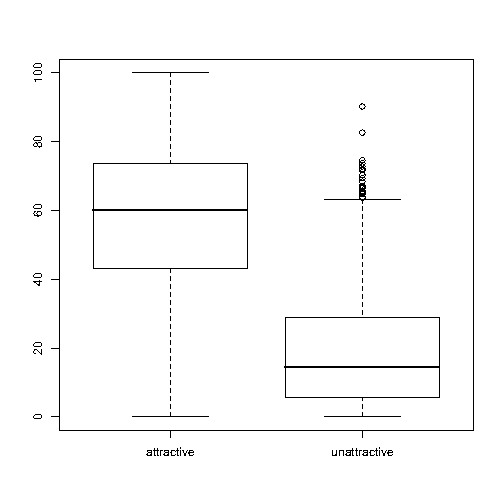
\includegraphics[width=80mm]{Rplot.pdf}\caption{Percentage of attractive friends of attractive/unattractive members}\label{fig: perc att}
\end{center}
\end{figure}

\begin{figure}
\begin{center}
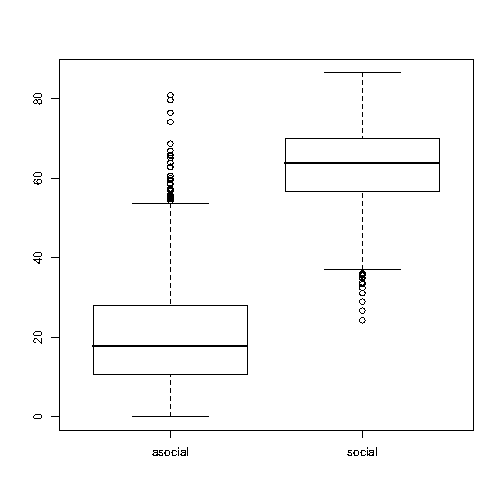
\includegraphics[width=80mm]{Rplot_soc.pdf}\caption{Percentage of social friends of social/asocial members}\label{fig: perc social}
\end{center}
\end{figure}


\subsubsection{Puzzle}

Several studies point to the fact that the growth of a community is highly dependent on its clustering coefficient.
This coefficient is defined as the ratio of closed to open triads in the friendship subgraph
induced by the members of a community.

\begin{figure}
  \begin{center}
    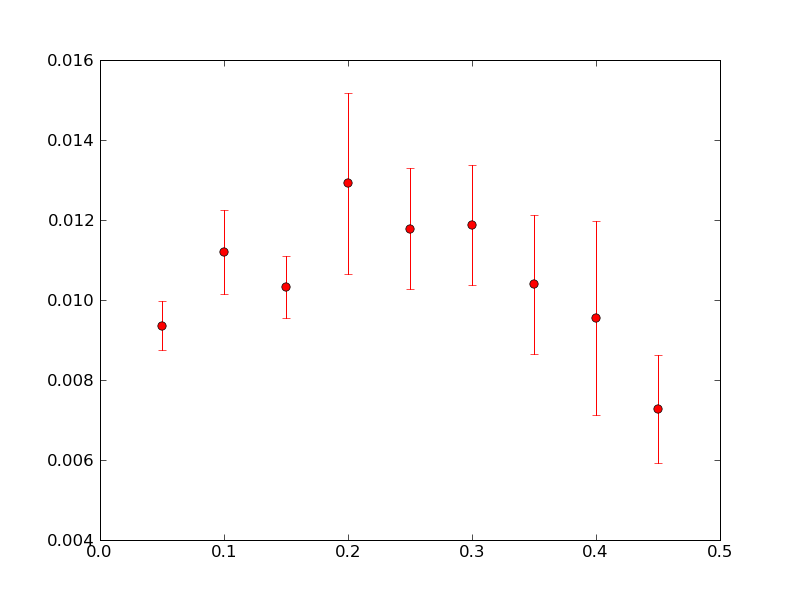
\includegraphics[width=8cm]{first.png}
    \caption{Community growth rates vs. ratio of closed to open triads: $1^{\rm st}$ snapshot}\label{fig:edge-a}
    \end{center}
\end{figure}


In Backstrom et al. paper \cite{group_formation}, the authors observe that if a community is highly connected, then it is less probable to grow.  This result is in contrast to the empirical evidence \cite{group_formation}  that suggests that a person is more probable to join a community,  if his/her friends inside the community are more interconnected.


\begin{figure}
  \begin{center}
    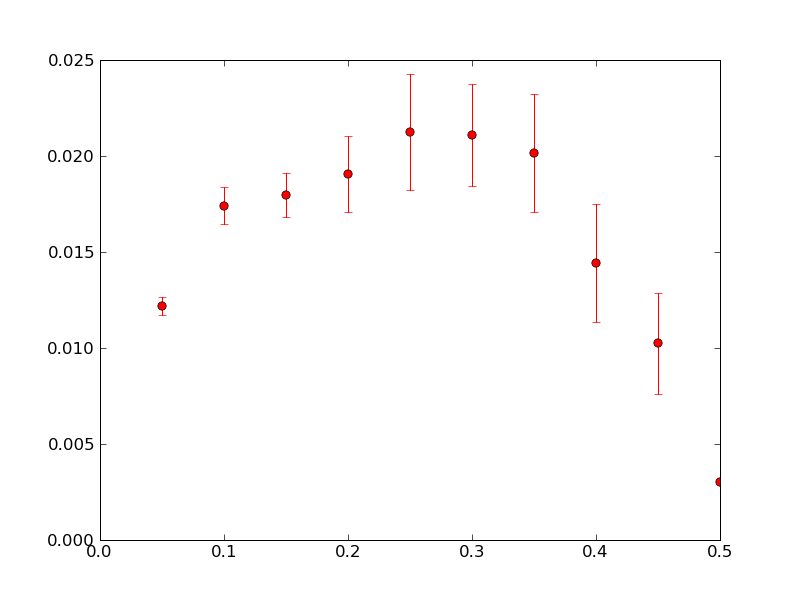
\includegraphics[width=8cm]{second.png}
    \caption{Community growth rates vs. ratio of closed to open triads: $2^{\rm nd}$ snapshot}\label{fig:edge-b}
    \end{center}
\end{figure}


In Figures \ref{fig:edge-a}-\ref{fig:edge-f}, for each snapshot, we plot the communities growth rates  as a function of their clustering coefficient.  Communities are binned together with respect to clustering coefficient. The growth rate is  decreasing for the communities that have clustering coefficients  higher than $0.3$, especially for the first two snapshots.  On the other hand, the number of communities  with large clustering coefficient  is much smaller than the ones with small clustering coefficient.

\begin{figure}
  \begin{center}
    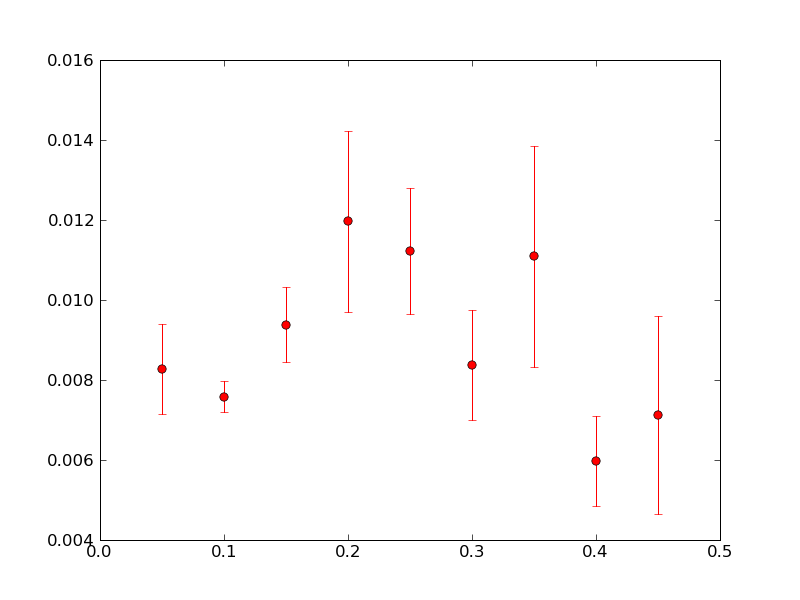
\includegraphics[width=8cm]{third.png}\label{fig:edge-c}
    \caption{Community growth rates vs. ratio of closed to open triads: $3^{\rm rd}$ snapshot}
    \end{center}
\end{figure}




In order to understand the relationship between  the clustering coefficient and the growth of a community, we divided 
the communities into two groups: $\mathcal{C}_h$ and $\mathcal{C}_l$, i.e., those that have  a clustering coefficient higher than the average, and those that have a  clustering coefficient less than the average. 

\begin{figure}
  \begin{center}
    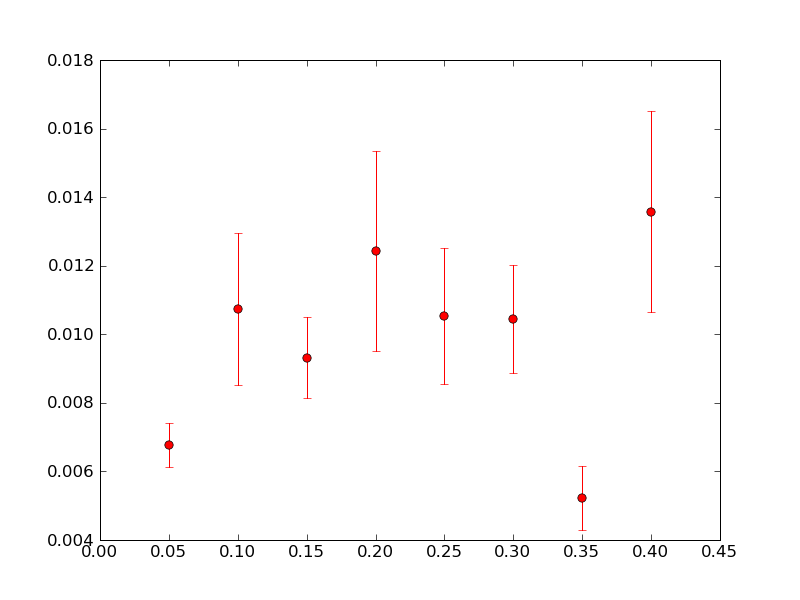
\includegraphics[width=8cm]{fourth.png}\label{fig:edge-d}
    \caption{Community growth rates vs. ratio of closed to open triads: $4^{\rm th}$ snapshot}
    \end{center}
\end{figure}




For each community $\Cc$, we computed the percentage of people in the fringe that only have one friends inside the community, i.e., 
\[
\frac{|\{x\in\mathcal{F} : \; x \textmd{ has only one friend in } \mathcal{C} \}|}{|\mathcal{F}|},
\]
and took the average among $\mathcal{C}_l$ and $\mathcal{C}_h$ separately. 
We found that for communities in $\mathcal{C}_l$ the average of this ratio is $86.6\%$, while for $\mathcal{C}_h$ it is
$76.9\%$.
Thus in the fringe of highly connected communities, on average, there are fewer people that have only one friend inside the community. Then we computed the probability 
of joining a community from its fringe for those who have only one friend inside. We took the average over $\mathcal{C}_l$ and $\mathcal{C}_h$ separately. 
The average probability of joining for such users among $\mathcal{C}_h$ communities turned out to be $8.4\times10^{-5}$, while the average of the same 
quantity for communities in $\mathcal{C}_l$ was $15.8\times 10^{-5}$ which is about two times  more. Therefore, since the majority of fringe consists of those who have only one friend inside, this partly describes the dichotomy. In other words the growth behavior  of a community is mainly determined by those in the fringe that have only one friend inside, because they are the majority of the fringe members; On the other hand, our empirical results suggest that these people are less probable to join a community if its is highly connected. 

\begin{figure}
  \begin{center}
    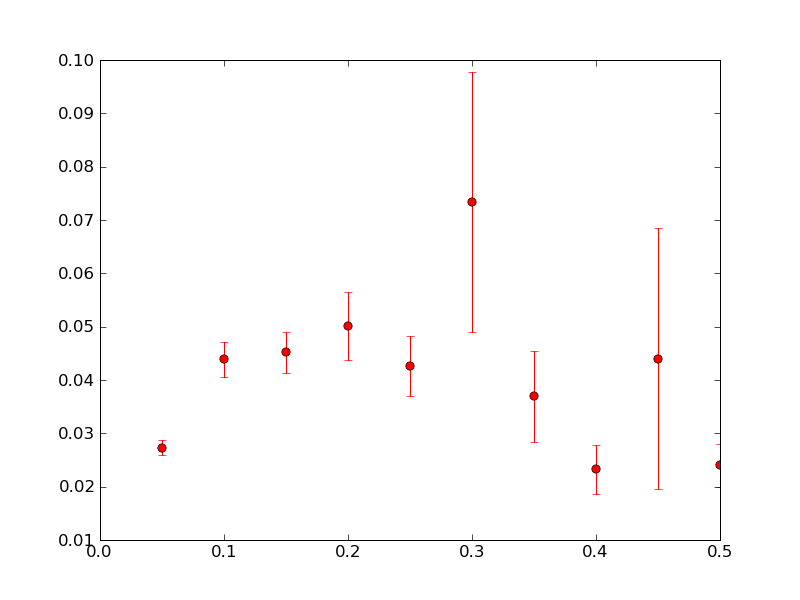
\includegraphics[width=8cm]{fifth.png}\label{fig:edge-e}
    \caption{Community growth rates vs. ratio of closed to open triads: $5^{\rm th}$ snapshot}
    \end{center}
\end{figure}


\begin{figure}
  \begin{center}
    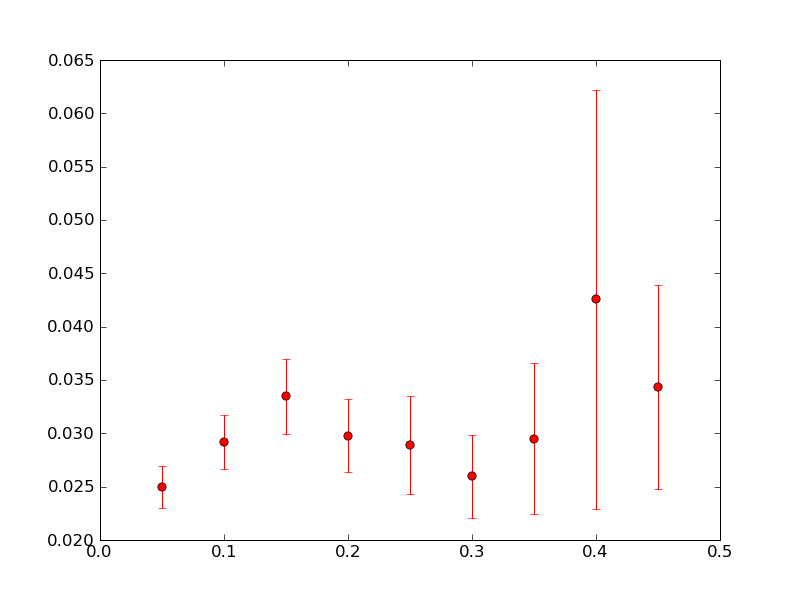
\includegraphics[width=8cm]{sixth.png}
    \caption{Community growth rates vs. ratio of closed to open triads: $6^{\rm th}$ snapshot}\label{fig:edge-f}
    \end{center}
\end{figure}



%\newpage
%\subsection{Simulation}
%
%In this section we propose a simple model for simulating the evolution of communities through time. First we observe the evolution of a community during some initial time period, and label its members as attractive and unattractive. Then to each member of the fringe we assign a probability $p_j$, the probability of joining the community, as follows
%\[
%p_{j} = \frac{1+C_{\rm a}N_a+C_{\rm una}N_{\rm una}}{1+C_0+C_{\rm a}N_a+C_{\rm una}N_{\rm una}},
%\]
%where $N_a$ is number of attractive friends of this member inside the community, and $N_{\rm una}$ is its number of unattractive friends. Also $C_0$, $C_{\rm at}$, and $C_{\rm una}$ are constants. In our simulations, after trying to find the parameters that fit the data, we used $C_0 = 250$, $C_{\rm a} = 2$, and $C_{\rm una}=1$, which seemed to give the best results. Although the model can predict all the
%non-growing communities correctly, it could predict only about half of the growing communities as growing. We would like to try different models in order to predict the growth.
%
\subsection{Further study of attractive people}
Let us focus on our measure \emph{attractivity} to understand more about what it really represents in the community
and its effects on growth.

\begin{itemize}
\item Are recent members of the community mostly attractive?
\end{itemize}

In Table \ref{table:rec}, for each snapshot,  we show what percentage of the people who
have joined the community in the previous snapshot are attractive.
 Especially for the first three snapshots, where
time between the snapshots are about a week, almost half of the recent members of the community are 
attractive. Given the fact that the attractive members in a community are much less than the unattractive 
ones, the recent members are more likely to be attractive.

\begin{table}[htdp]
\caption{Average percentage of attractive people among the people who have just joined}
\begin{center}
\begin{tabular}{|c|c|c|c|c|c}
\hline
snapshot & 2 & 3 & 4 & 5 \\ \hline
average percentage of   & 0.524 & 0.510 & 0.550 & 0.382 \\
attractive people  &  &  & &  \\ \hline
\end{tabular}
\end{center}
\label{table:rec}
\end{table}

%\begin{figure}
%\begin{center}
%\includegraphics[width=120mm]{rec_att.pdf}\caption{Distribution of attractivity of new comers}\label%{fig:rec_att}
%\end{center}
%\end{figure}

\begin{itemize}
\item Are there people who are always attractive?
\end{itemize}

Among the first four snapshots, for each person in a community, we computed the number of snapshots
he/she has been attractive. Table  \ref{table:all} shows the number of people that were attractive in just one snapshot, two snapshots etc.
So, we can conclude that the most people don't stay attractive for a long time.

\begin{table}[htdp]
\caption{Frequency of being  attractive for difference people}
\begin{center}
\begin{tabular}{|c|c|c|c|c|}
\hline
number of snapshots & 1 & 2 & 3 & 4  \\ \hline
number of people  & 29,255 & 6,171 & 3,954 & 34 \\ \hline
\end{tabular}
\end{center}
\label{table:all}
\end{table}%

\begin{itemize}
\item Is attractiveness of a person group-dependent?
\end{itemize}

One question to ask is whether knowing that a person is considered active in a group increases the chance of $v$ being attractive in other groups that contain $v$ as well. Similarly, does being unattractive in one community makes it more probable to be unattractive in other groups too. Let a person $v\in\Vc$ belong to $n_v$ different communities, $\mathcal{C}_1,\ldots,\mathcal{C}_{n_v}$. The vector  $(a_v(\Cc_1),\ldots,a_v(\Cc_{n_v})$ represents attractiveness of $v$ in these communities. For each person $v\in\Vc$ define 
\begin{align}
p_v\triangleq\max\left(\frac{\sum\limits_{i=1}^{n_v} a_v(\Cc_i)}{n_v},1-\frac{\sum\limits_{i=1}^{n_v} a_v(\Cc_i)}{n_v}\right).
\end{align}
If $v$ belongs to 5 communities and its attractiveness status vector is $(0,1,1,0,1)$  or $(1,0,0,1,0)$ in both cases $p_v=60\%$. From our data, we looked at  $\frac{1}{n}\sum_i p_i  $. Table \ref{table:glob} shows strong correlation among the variables.

\begin{table}[htdp]
\caption{Attractivity of a user in different communities}
\begin{center}
\begin{tabular}{|c|c|c|c|c|}\hline
snapshot & 1 & 2 & 3 & 4  \\ \hline
ratio  & 0.916 & 0.925 & 0.989 & 0.89 \\ \hline
\end{tabular}
\end{center}
\label{table:glob}
\end{table}%





\section{Conclusion}

We have studied six snapshots of about $2000$ communities from the online social network LiveJournal. Our main goal was to find the structural features of communities that can help us with the prediction of growth. We have found that the percentage of \emph{attractive} members of a community in a short time interval, has a strong correlation by its growth rate in the future. We also tried to measure the correlation between the growth and some structural properties of the communities such as  clustering coefficient and average degree. None of them showed evidence of strong correlation.

When we focused on  attractiveness, we found that people are attractive for a short period, and it is not something intrinsic to the community. Also among the newly joined members, the percentage of attractive members is much higher. On the other hand, people are likely to be attractive in different communities that they belong to at the same time.  All these gives us the sense that attractiveness is strongly related to being active.

\subsection{Future Work}

We believe that the percentage of \emph{attractive} members of a community can be a good way to
predict  community growth. The next step is to understand this notion of being \emph{attractive} more 
thoroughly. Does our hypothesis of its being strongly related to activeness of a member is true? 
Can we relate it to some inherent structure of a community? 

Another future work is to come up with a model that predicts the growth of a community using the attractiveness measure. In order to examine the consistency of our results, applying similar analysis to user-defined communities in another social network  is also crucial.

\section*{Acknowledgments}

We would like to give our thanks to Professor Andrea Montanari for providing us with a lot of  constructive feedback during this work.


\begin{thebibliography}{99}

\bibitem{social_ref}
J.~Coleman, Foundations of Social Theory, Harvard, 1990.

\bibitem{group_formation} L.~Backstrom, D.~Huttenlocher, J.~Kleinberg, X.~Lan, ``Group formation in large social networks: membership, growth, and evolution'', Proc.~of the $12^{\rm th}$ {\it ACM SIGKDD international conference on Knowledge discovery and data mining}, 2006

\bibitem{book_anova}
M.H.~Kutner, C.J.~Nachtsheim, J. Neter, W.~Li, \emph{ Applied Linear Statistical Models} (5th ed.), McGraw-Hill/Irwin.

\bibitem{kumar_tomkins} R.~Kumar, J.~Novak, and A.~Tomkins, ``Structure and
evolution of online social networks." In $12^{\rm th}$ KDD, pages~611-617, 2006.

\bibitem{LKF} J.~Leskovec, J.~Kleinberg, C.~Faloutsos. ``Graph
evolution: Densification and shrinking diameters." ACM
TKDD, 1(1):2, 2007.

\bibitem{micro_evol} J.~Leskovec, L.~Backstrom, R.~Kumar, A.~Tomkins.  ``Microscopic Evolution of Social Networks", ACM SIGKDD, 2008. 

\bibitem{newman} M.E.J.~Newman. ``Detecting community structure in networks." \emph{The European Physical Journal B}, 38:321-330, 2004.

\bibitem{danon} L.~Danon, J.~Duch, A.~Diaz-Guilera, A.~Arenas. ``Comparing community structure identification." \emph{Journal of Statistical Mechanics: Theory and Experiment}, 29(09):P09008, 2005.

\bibitem{www10}  J.~Leskovec, K.~Lang, M.~Mahoney.``Empirical Comparison of Algorithms for Network Community Detection" ACM WWW {\it International conference on World Wide Web}, 2010. 

\bibitem{define_comm} F.~Radicchi, C.~Castellano, F.~Cecconi, V.~Loreto,
D.~Parisi. ``Defining and identifying communities in networks."
{\it Proceedings of the National Academy of Sciences of the
United States of America}, 101(9):2658-2663, 2004.

\bibitem{clustering}
D.J.~Watts, \emph{Small Worlds: The Dynamics of Networks Between Order and Randomness,} Princeton Univ. Press, Princeton, NJ, 1999.

\end{thebibliography}


\end{document}
